\documentclass[12pt, titlepage, letterpaper]{article}
%\documentclass[12pt, letterpaper, titlepage]{article}

\usepackage{amsmath}
\usepackage{booktabs}
\usepackage{amsthm}
\usepackage{graphicx}
\usepackage[margin=1in]{geometry}
\usepackage{hyperref}
\hypersetup{colorlinks = true, linkcolor = blue, citecolor=blue, urlcolor = blue}
\usepackage{natbib}
\usepackage{enumitem}
\usepackage{setspace}


\usepackage[]{lineno}
\linenumbers*[1]
% %% patches to make lineno work better with amsmath
\newcommand*\patchAmsMathEnvironmentForLineno[1]{%
 \expandafter\let\csname old#1\expandafter\endcsname\csname #1\endcsname
 \expandafter\let\csname oldend#1\expandafter\endcsname\csname end#1\endcsname
 \renewenvironment{#1}%
 {\linenomath\csname old#1\endcsname}%
 {\csname oldend#1\endcsname\endlinenomath}}%
\newcommand*\patchBothAmsMathEnvironmentsForLineno[1]{%
 \patchAmsMathEnvironmentForLineno{#1}%
 \patchAmsMathEnvironmentForLineno{#1*}}%

\AtBeginDocument{%
 \patchBothAmsMathEnvironmentsForLineno{equation}%
 \patchBothAmsMathEnvironmentsForLineno{align}%
 \patchBothAmsMathEnvironmentsForLineno{flalign}%
 \patchBothAmsMathEnvironmentsForLineno{alignat}%
 \patchBothAmsMathEnvironmentsForLineno{gather}%
 \patchBothAmsMathEnvironmentsForLineno{multline}%
}

% control floats
\renewcommand\floatpagefraction{.9}
\renewcommand\topfraction{.9}
\renewcommand\bottomfraction{.9}
\renewcommand\textfraction{.1}
\setcounter{totalnumber}{50}
\setcounter{topnumber}{50}
\setcounter{bottomnumber}{50}

\newcommand{\jy}[1]{\textcolor{blue}{JY: #1}}
\newcommand{\eds}[1]{\textcolor{red}{EDS: (#1)}}
\newcommand{\mc}[1]{\textcolor{green}{MC: (#1)}}

% NOTE: To produce blinded version, replace "0" with "1" below.
\newcommand{\blind}{1]}

\begin{document}
%\maketitle

\title{\bf Nonparametric Bootstrap Kolmogorov-Smirnov Goodness-of-Fit Test for
  Marginal Distributions of Stationary Time Series}
\if0\blind
{
  \author{Mathew Chandy, %\\
%   \href{mailto:mathew.chandy@uconn.edu}
%   {\nolinkurl{mathew.chandy@uconn.edu}}\\
  Elizabeth Schifano\\
  Jun Yan, %\\
  Xianyang Zhang\\
} \fi


\maketitle


\begin{abstract}

The Kolmogorov-Smirnov (KS) statistic is widely used to test if a sample is
from a given distribution. This study demonstrates how non-parametric 
block bootstrap can be 
used to approximate the KS statistic in situations where parameters are 
not specified and the data are serially dependent. We demonstrate the 
theoretical justication for this method, then through simulation we verify that
it holds it size under the null distribution and is powerful when the null 
hypothesis is false. Finally, we demonstrate applications of the method to
precipitation data from three airports and Microsoft stock returns.

\bigskip
\noindent{\sc Keywords}:
bias-correction; 
dependent data; 
time series. 
\end{abstract}

\doublespace 


\section{Introduction}
\label{sec:intro}

\jy{Start from the need for KS test for stationary series; review existing works
  and identify the gap; summarize the contribution.}

The Kolmogorov-Smirnov (KS) test is a useful goodness-of-fit statistic. 
Let $X_1, ..., X_n$ be a random sample of size~$n$ from some continuous
distribution. The null hypothesis $H_0$ is that $X_i$'s follow the
hypothesized distribution~$F$.
Let $F_n(t) = \sum_{i=1}^n I(X_i \le t) / n$ be the empirical cumulative
distribution function of the sample, where $I(\cdot)$ is the indicator
function. The KS test statistic takes the form
\begin{equation}
  \label{eq:ks_standard}
  T_n = \sqrt{n} \sup_x | F_{n}(x) - F(x) |.
\end{equation}


The statistic 
can be used to see if a population follows a hypothesized distribution and has 
and can be applied to a variety of fields. It has
been used to analyze the random distribution of cosmic microwave background 
radiation \citep{naess2012application}. \citet{zeimbekakis2022misuses} reviews
some of the common misuses of the one-sample KS test. One of the most common 
misuses of the KS test is when
the hypothesized distribution has unspecified parameters. 
\citet{babu2004goodness} approaches this scenario using basic 
non-parametric bootstrap. There is also the scenario where the data are serially
dependent, which \citet{zeimbekakis2022misuses} partially remedies with 
semi-parametric
bootstrap. The last scenario \citet{zeimbekakis2022misuses} discusses is that
where both the hypothesized 
distribution has unspecified parameters and the data are 
serially dependent. \citet{zeimbekakis2022misuses}'s remedy for
this scenario also uses semi-parametric bootstrap.


A complete remedy for KS tests with serially dependent data is
a challenging task. The null distribution depends on the structure of the serial
dependence, which can be arbitrary in practice. A parametric bootstrap procedure
would demand a specification for a model for the dependence, whereas the primary 
interest
is to test the marginal distribution of the stationary series. A bias 
correction
for block bootstrap similar to what \citet{babu2004goodness} did for basic
bootstrap had not yet been shown.  This study aims to resolve this gap by 
demonstrating a bias 
correction
for non-parametric block bootstrap to use when the hypothesized distribution
has unspecified parameters and the data are serially dependent.


The rest of the paper is outlined as follows: Section~\ref{sec:methods} reviews
block bootstrap procedure and demonstrates the basis for bias correction for
the non-parametric block bootstrap KS test. In Section~\ref{sec:simu}, we first 
assess whether the KS
test holds its size; that is, does the test fail to reject the null hypothesis
when it is true. In the second part of Section~\ref{sec:simu}, we 
evaluate the 
test's power; that is, does the test reject the null hypothesis when it is 
false. We show practical applications of this method in Section~\ref{sec:real}.
First, we apply the method to test if annual maximums of hourly precipitation
in three U.S. airports follows the GEV distribution in 
Subsection~\ref{sec:precipitation}.
Then, we test if Microsoft stock return data follows the Normal or the Student's
$t$ distribution in Subsection~\ref{sec:microsoft}.
Finally, we end with 
concluding remarks in Section~\ref{sec:conclusion}.


\section{Methods}
\label{sec:methods}


Consider a stationary time series $\{X_t: t = 1, \ldots, n\}$ with length~$n$.
We are interested in testing whether or not $X_t$ follows a distribution in a
parametric family of distribution~$F$ indexed by a parameter
vector~$\theta$. That is, the null hypothesis is
\[
  H_0: X_t \sim F(\cdot \mid \theta), \quad t = 1, \ldots, n,
\]
for some unspecified parameter $\theta$.
The alternative hypothesis $H_A$ is that the marginal distribution of $X_t$ does
not follow~$F$ for any parameter value~$\theta$. This is a challenging situation
both the parameters and the serial dependence structure are unknown.


First, let us consider how the KS statistic is typically computed for a sample
with no dependence structure.
Let $\hat\theta_n$ denote the fitted parameters for the hypothesized 
distribution fitted onto $X_t$, and let 
$F_n$ denote the empirical distribution function based on $X_1,...,X_n$
Let
\begin{equation*}
Y_n(x; \hat\theta) = \sqrt{n}(F_n(x) - F(x; \hat\theta_n)).
\end{equation*}
Then, the
goodness of fit statistic is 
\begin{equation*}
T_n := \sup_x|Y_n(x; \hat\theta)|.
\end{equation*}

We note that
\begin{equation*}
Y_n(x; \hat\theta) = \sqrt{n}(F_n(x) - F(x)) - 
\sqrt{n}(F(x; \hat\theta_n) - F(x)),
\end{equation*}
where $F(x)$ is the true cdf (under the null $F(x) = F(x, \theta_0)$ for some
true parameter $\theta_0$).


Let us first consider the case where $X_i$'s are i.i.d. Denote by $F^{(b)}_n$ 
the empirical distribution of the $b$th bootstrap sample and let
$\hat\theta^{(b)}_n$ be the parameter estimate based on the $b$th bootstrap 
sample. 
Using the bootstrap (asymptotic) theory, we can approximate the distribution of
\jy{need references to back up}
$\sqrt{n}(F_n(x) - F(x))$ and $\sqrt{n}(F(x; \hat\theta_n) - F(x))$
by that of $\sqrt{n}(F^{(b)}_n(x) - F_n(x))$
and
$\sqrt{n}(F(x; \hat\theta^{(b)}_n) - F(x; \hat\theta_n))$, respectively.
Therefore, if we define
\begin{align*}
Y^{(b)}_n(x) &= \sqrt{n}(F^{(b)}_n(x) - F_n(x)) - 
               \sqrt{n}(F(x; \hat\theta^{(b)}_n) - F(x; \hat\theta_n)) \\
             &= \sqrt{n}(F^{(b)}_n(x) - F(x; \hat\theta^{(b)}_n)) - 
               \sqrt{n}(F_n(x) - F(x; \hat\theta_n)),
\end{align*}
then $T^{(b)}_n := \sup_x|Y^{(b)}_n(x)|$ is the bootstrap statistic that is 
expected
to approximate the distribution of $T_n$. We note that the term
$\sqrt{n}(F_n(x) - F(x; \hat\theta_n))$ is exactly the bias term considered in 
\citet{babu2004goodness}.


We now consider the case where $X_i$'s are realizations from a time series and
$X^{(b)}_1,...,X^{(b)}_n$ are generated by block bootstrap for 
$b \in \{1, \ldots, B\}$.  
Block-bootstrap can be done with overlapping or moving blocks.
Define 
moving blocks (assuming $l > 1$) as:
\begin{equation*}
Z_j =
    \begin{cases}
        \{X_j, \ldots, X_{j + l - 1}\}, & j = 1, \dots, n - l + 1,\\
        \{X_j, \ldots, X_n, X_1, \ldots, X_{j-n+l-1}\}, & j = n - l
        + 2 ,\dots, n.
    \end{cases}
\end{equation*}
A common 
function for block size that is considered optimal is 
$l = \lceil n^{1/3} \rceil$ \citep{buhlmann1999block},  
which was adopted in this study.


We then use bootstrap to approximate the distribuition of
the KS statistic under $H_0$. In this case, we can 
use the distribution of $\sqrt{n}(F^{(b)}_n(x) - E[F^{(b)}_n(x)])$
as an approximation of the distribution of
$\sqrt{n}(F_n(x) - F(x))$,
and the distribution of 
$\sqrt{n}(F(x; \hat\theta^{(b)}_n) - F(x; E[\hat\theta^{(b)}_n]))$ to
approximate $\sqrt{n}(F(x; \theta_n) - F(x))$'s distribution.


We can compute $E[F^{(b)}_n(x)]$ and
$E[\hat\theta^{(b)}_n]$ numerically (they can also be computed analytically, 
depending on the types of block bootstrap we use). One can compute 
$F^{(b)}_n$ 
and $\hat\theta^{(b)}_n$ based on
the $b$th bootstrap sample. Then
$E[F^{(b)}_n(x)] \approx \frac{1}{B}\sum_{b = 1}^BF^{(b)}_n(x)$, and
$E[\hat\theta^{(b)}_n] \approx \frac{1}{B}\sum_{b = 1}^B\hat\theta^{(b)}_n$.
In this case, we can define
\begin{align*}
  Y^{(b)}_n(x) &= \sqrt{n}(F^{(b)}_n(x) - E[F^{(b)}_n(x)]) - 
             \sqrt{n}(F(x; \hat\theta^{(b)}_n) - F(x; E[\hat\theta^{(b)}_n)]) \\
           &= \sqrt{n}(F^{(b)}_n(x) - F(x; \hat\theta^{(b)}_n)) -
             \sqrt{n}(E[F^{(b)}_n(x)] - F(x; E[\hat\theta^{(b)}_n])),
\end{align*}
and $T^{(b)}_n = \sup_x|Y^{(b)}_n(x)|$. Each $T_n^{(b)}$,
$b =1, \ldots, B$, is considered a draw from a distribution that approximates
the distribution of $T_n$. Therefore, the p-value of the observed statistic
$T_n$ can be assessed by positioning it agains the empirical distribution of
$T_n^{(b)}$, $b = 1, \ldots, B$.


In summary, the procedure of the nonparametric block bootstrap test is 
summarized as follows.
\jy{Whrere is the 'block' part?}
\begin{enumerate}
\item
  Generate $X^{(b)}_1,...,X^{(b)}_n$ by applying moving block bootstrap 
  on the original sample as
  defined previously.
\item
  Fit $F_\theta$ to $X^{(b)}_1,...,X^{(b)}_n$ and obtain estimate 
	$\hat\theta^{(b)}_n$ of $\theta$.
\item
  Obtain the empirical distribution function $F^{(b)}_n$ of
  $X^{(b)}_1,...,X^{(b)}_n$. 
\item
  Calculate bootstrap KS statistic
  \[
    T^{(b)}_n = \sup_x | \sqrt{n}\left(F^{(b)}_n(x) 
    - F(x; \hat\theta^{(b)}_n)\right) - B_n(x) |.
  \]
  where 
  $B_{n}(x) = \sqrt{n}(E[F^{(b)}_n(x)] - 
  F(x; E[\hat\theta^{(b)}_n]))$ is the known
  bias term.
\item
  Repeat the previous steps a large number $B$ times and use the empirical
  distribution of $T^{(b)}_n$ to approximate the null distribution of the observed
  statistic. 
\end{enumerate}


The p-value of the block bootstrap KS test can be computed
as $p = \#\{T^{(b)}_n > T_n\} / B$ for 
$b \in \{1, \ldots, B\}$.

\section{Simulation Studies}
\label{sec:simu}

If we can show that the test correctly fails to reject $H_0$ under the null
distribution, and correctly rejects $H_0$ for an alternate distribution, we can
state that the method works.


\subsection{Size}
We first must evaluate whether this method works when $H_0$ is true. To
test this, we can
generate a simulated sample $X_t$ with a certain marginal distribution 
$F_\theta$,
and use our method to test if $X_t$ indeed has the marginal distribution $F$ 
with some unknown $\theta$. If the test holds its size, the 
p-value
of the test should be uniformally distributed between 0 and 1. We must try the
method with different marginal distributions to ensure that it is robust.
In order for the method to work, a large sample size may be necessary. 


\jy{Give details on how the data were generated. Are these enough infomation for
  people reproduce the results? I'd suggest that we use Kendall's tau to measure
  the serial dependence. }


We generated time series with marginal distributions $N(8, 8)$ and
\jy{why choose these two distributions?}\mc{addressed}
$\Gamma(8, 1)$, lag-1 autocorrelation $\phi \in \{-.4, -.2, 0, .2, .4\}$, and
sample size $n \in \{100, 200, 400, 800, 1600, 3200\}$. These distributions
were chosen to compare results on normal and non-normal
error structures, and the parameters were chosen so that the distributions
have the same mean 8 and variance 8. To generate 
For the purposes of 
evaluating if the test holds it size, when $X_t \sim N(8, 8)$, we tested that the 
marginal distribution family is normal, and when $X_t \sim \Gamma(8, 1)$, we tested
that the marginal distribution family is gamma. For the block bootstrap step,
we used $B = 1000$ and $l = \lceil n^{1/3} \rceil$.
For each setting for $F$, $\phi$, and $n$, we replicate the method 1000 times 
to get the distribution of the p-values 
for the test when applied to samples from the same data generating process.


Using the \textsl{qqplotr} and \textsl{ggplot2} packages 
\citep{qqplotr, ggplot2},
we constructed Q-Q plots of the distribution of the p-values to see if they are
uniformly distributed. If the distribution of the p-values is uniform, this 
indicates that under the null hypothesis, our method will only reject the $H_0$
at a rate of $\alpha$.
A zoomed in plot for probabilities between 0 and 0.1 is
also provided, as
that is the most common range for significance levels $\alpha$. 
%We can also
%compute the rate of rejection $\#P < \alpha$ for different values of
%$\alpha$, as well as a confidence interval
%for this proportion.

\jy{Reduce width of  the panel title section. Reduce the font size of the
  labels. Generate the figures with the right size in mind. Use whole textwidth.}
  
\begin{figure}[tbp]
  \centering
  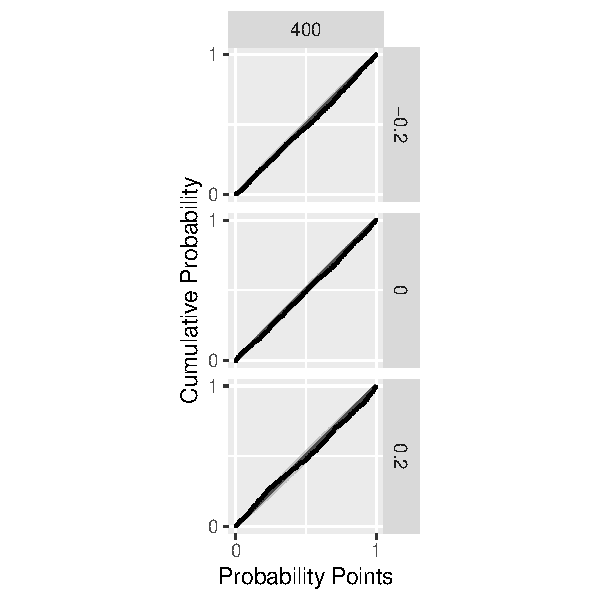
\includegraphics[width = \textwidth]{figures/normal}
  \caption{A Q-Q plot of the p-values testing that a distribution
  generated from a $N(8,8)$ data generating process is normal.}
  \label{fig:normal}
\end{figure}

\begin{figure}[tbp]
  \centering
  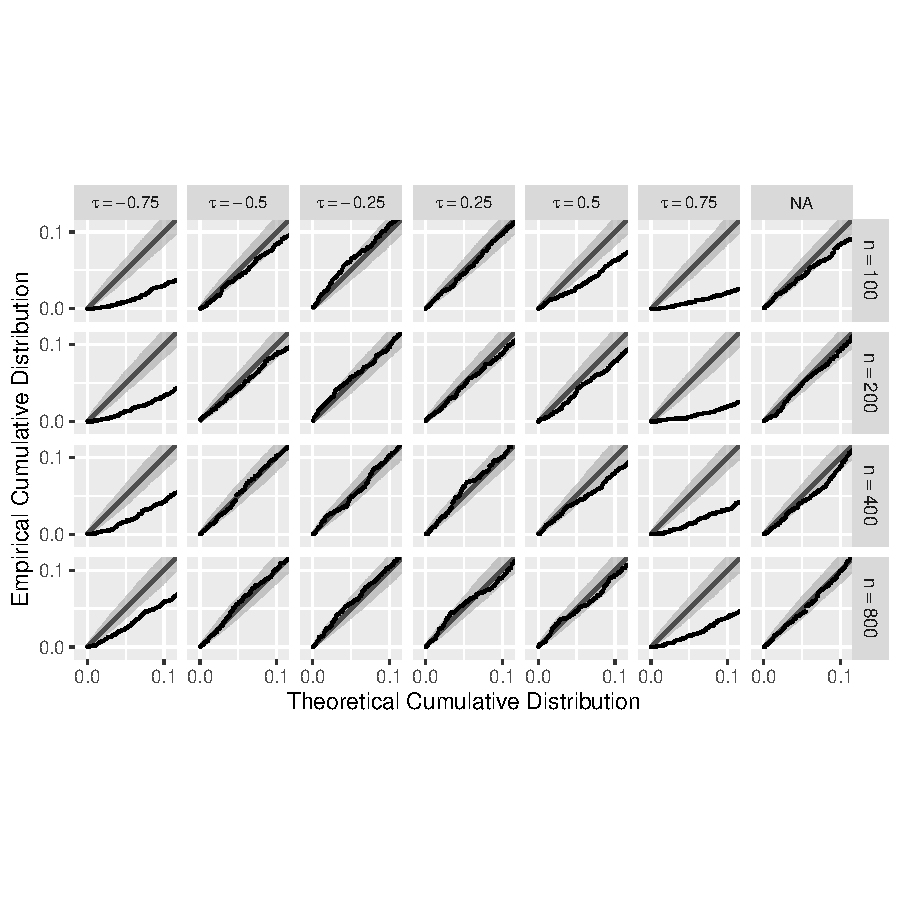
\includegraphics[width = \textwidth]{figures/zoom_normal}
  \caption{A Q-Q plot of the p-values displayed in Figure~\ref{fig:normal} zoomed in to 
  probabilities between 0 and
  0.1}
  \label{fig:zoom_normal}
\end{figure}

\begin{figure}[tbp]
  \centering
  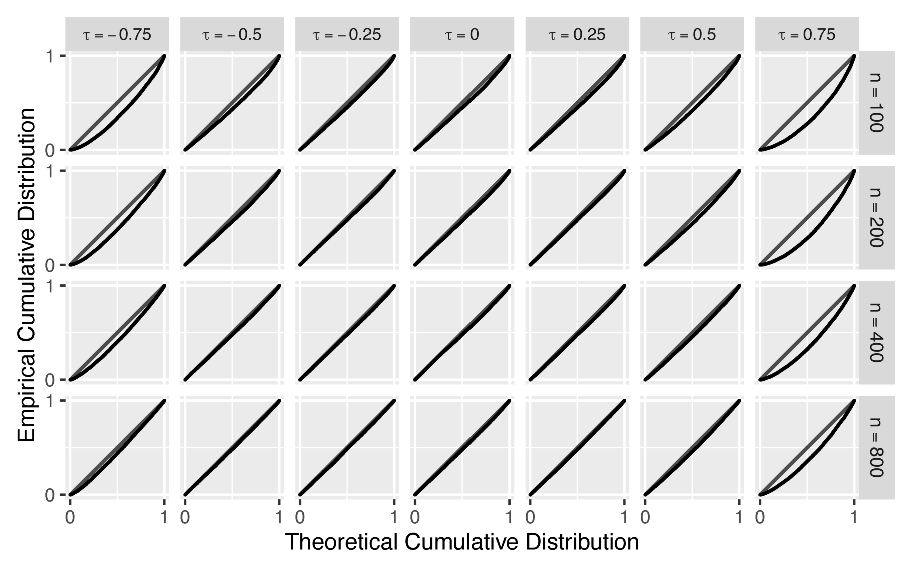
\includegraphics[scale=1]{figures/gamma}
  \caption{A Q-Q plot of the p-values testing that a distribution
  generated from a $\gamma(8,1)$ data generating process is gamma distributed.}
  \label{fig:gamma}
\end{figure}

\begin{figure}[tbp]
  \centering
  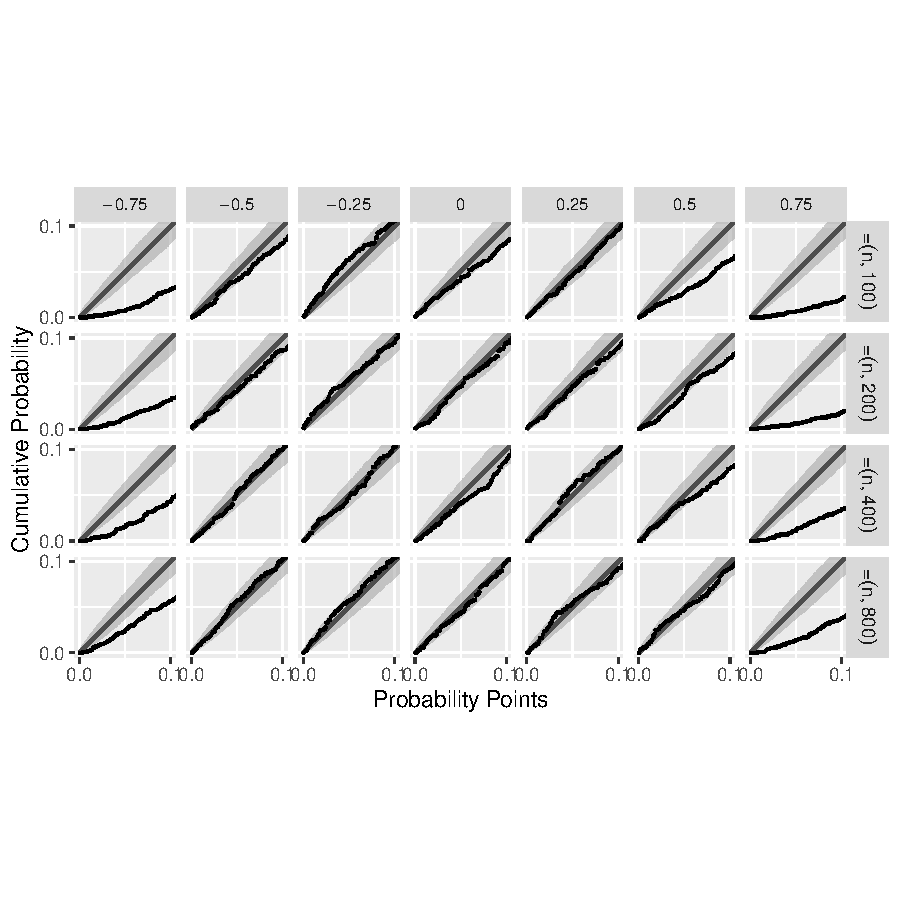
\includegraphics[scale=1]{figures/zoom_gamma}
  \caption{A Q-Q plot of the p-values displayed in Figure~\ref{fig:gamma} zoomed in to 
  probabilities between 0 and
  0.1}
  \label{fig:zoom_gamma}
\end{figure}

From Figures~\ref{fig:normal} and \ref{fig:gamma}, we can observe that 
although the p-values do not appear to be 
completely aligned with the line
in the Q-Q plots for smaller sample sizes like $n = 100$ or $200$, they match
the lines very closely for $n = 1600$ and $3200$. More importantly, almost
all of the p-values appear to be within the confidence bands when looking at the
plots zoomed in to probabilities between 0 and 0.1 in 
Figures~\ref{fig:zoom_normal} and \ref{fig:zoom_gamma}, and as stated 
before, 
researchers are unlikely to choose significance levels above 0.1. 


Under $H_0$, the p-values for the non-parametric block bootstrap KS test are
uniformly distributed. This is an indication that our method 
holds its size and that we can expect the probability
of a type 1 error to be the significance level $\alpha$.


\subsection{Power}
We must also evaluate if this method works when $H_0$ is false. We can use
the block bootstrap KS test to test if some $X_t \sim F$ is generated from 
some other 
distribution $G$ with some unknown $\theta$. In this scenario, if the test is 
indeed powerful,
we would ideally want $\beta$ 
(or the probability of failed rejection under $H_A$) 
to be 0, but we
expect it to be generally low. Again, we must try the method with different
marginal distributions to ensure that it is robust.
We would then expect the distribution of p-values to be non-uniform, and the 
rate
of $\#P < \alpha$ to be high, meaning a higher density of low p-values.


Like we did to see if the test holds its size, we generated time series with 
marginal distributions $N(8, 8)$ and 
$\Gamma(8, 1)$, lag-1 autocorrelation $\phi \in \{-.4, -.2, 0, .2, .4\}$, and
sample size $n \in \{200, 400, 800\}$. However, 
to evaluate the test's power, when $X_t \sim N(8, 8)$, we tested that the 
marginal distribution family is gamma. Because the support of $N(8, 8)$ is
$(-\infty, \infty)$, but the support of $\Gamma(8, 1)$ is $(0, \infty)$, we used
the \textsl{truncdist} package \citep{truncdist} to truncate the series at 
values less than or equal to 0.
When $X_t \sim \Gamma(8, 1)$, we tested
that the marginal distribution family is normal. For the block bootstrap step,
we used $B = 1000$ and $l = \lceil n^{1/3} \rceil$.
For each setting for $F$, $\phi$, and $n$, we replicate the method $1000$ times 
to obtain a p-value $p_r$ for each $r \in \{1, \ldots, 1000\}$.


Given some significance level $\alpha$, we can compute a rejection rate 
$q = \#\{p_r < \alpha\} / 1000$ for $r \in \{1, \ldots, 1000\}$.
Additionally, we can construct a 95\% confidence interval for 
this rate. Below are tables containing rejection rates showcasing the 
differences when simulation settings are changed.

\jy{Clean up the tables. Use percentage for power. Keep three effective
  digits. Why are there so many decimal places? }
\mc{reduced number of digits}

\jy{The large number decimals in the old table: some numerical issues?}

\jy{Only three sample sizes will be enough. Sample size 800 or higher give
  power~1. Only report nominal size 0.05 would be ok. May consider presenting
  the intervals in a figure.}
\mc{only included three sample sizes and for alpha $=$ 0.05}


\jy{Consider presenting this in a graph. Try explaining the pattern.
  Keep the notations consistent: $n$ and n are different.}


\begin{figure}[tbp]
  \centering
  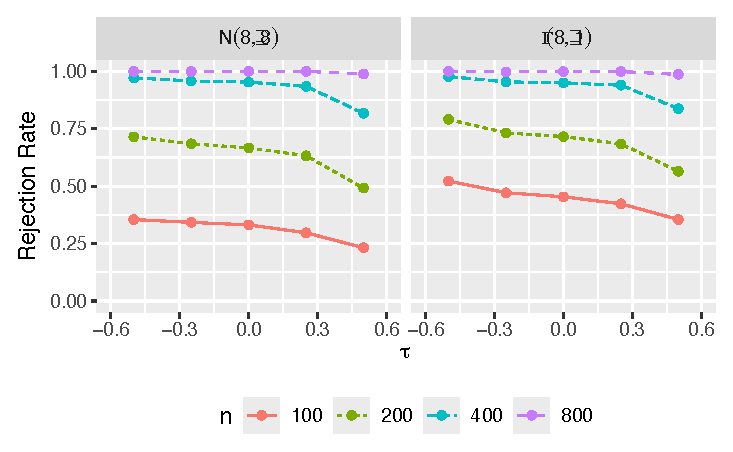
\includegraphics[scale=1]{figures/rr}
  \caption{A plot of the rejection rates as a function of $\tau$ for
 $n \in \{100, 200, 400, 800\}$ and marginal distribution 
 $\in \{N(8,8), \gamma(8,1)\}$.}
  \label{fig:rr}
\end{figure}


From 
Table~\ref{fig:rr}, 
the rejection rates are a little higher for $n = 200$, but they may still be 
drop below 50\% is the $\alpha = 0.1$. Once $n$ reaches 400, we can observe 
that the rejection rate
is consistently above 50\%. For larger sample sizes, the rejection rate is 
consistently above 90\%. We can also
observe that the rejection rate is slightly higher for the $\gamma(8, 1)$ sample 
than for 
the $N(8, 8)$. As the strength of the temporal dependence increases, the 
rejection rate decreases, and the rejection
rate appears to be slightly higher for negative temporal dependence versus 
positive temporal dependence values of the same strength.


The rejection rates for $n = 800$
are very 
high (almost 1), indicating that under $H_A$, the test is very powerful 
(low probability of failed rejection $\beta$) when a large enough
sample size is used.


\section{Real Data Analysis}
\label{sec:real}

\subsection{Precipitation in Mansfield Connecticut}
\label{sec:precipitation}
Annual maximums of hourly precipitation in inches time series data were 
retrieved 
from the Chicago Midway International Airport (MDW), New York LaGuardia 
International 
Airport (LGA),
and Los Angeles International Airport (LAX) stations from the 
National Oceanic and Atmospheric Administration. These stations were selected 
from places of importance in the three largest American cities. LGA and
MDW were chosen over John F. Kennedy and O'Hare as more data was available
from these stations. The data for MDW is from
1948 to 2014, the data for LGA is from 1948 to 2013, and the
data for LAX is also from 1948 to 2013. We can apply our method to
the precipitation time series from each of these locations to test if they
follow the
Generalized Extreme Value (GEV) distribution using the \textsl{evd} 
package \citep{evd}. Precipitation maximum series 
typically do follow the GEV distribution, so we expect to fail to reject the
null hypothesis.

\jy{No need for such small a table. Could plot the histogram and fitted density.}

% latex table generated in R 4.3.0 by xtable 1.8-4 package
% Sun Feb 25 12:46:58 2024
\begin{table}[ht]
\centering
\caption{P-values for testing that annual maximums of hourly 
            precipitation from the three airports follows the GEV distribution.} 
\label{table:precipitation}
\begin{tabular}{rrrr}
  \hline
 & block & basic & param \\ 
  \hline
MDW & 0.16 & 0.21 & 0.08 \\ 
  LGA & 0.44 & 0.55 & 0.48 \\ 
  LAX & 0.28 & 0.36 & 0.34 \\ 
   \hline
\end{tabular}
\end{table}


%\mc{https://hdsc.nws.noaa.gov/pfds/pfds_map_cont.html?bkmrk=ct}

As displayed in Table~\ref{table:precipitation}, using a significance level as 
high as .10 still results in a failed rejection
of the null hypothesis for each of the three tests that the respective 
time series follow the GEV distribution.

\subsection{Microsoft Stock Returns}
\label{sec:microsoft}

%\mc{https://www.nasdaq.com/market-activity/stocks/msft/historical}

We expect the marginal distribution of Microsoft stock returns to have a 
slightly
heavier tail than the normal distribution. Using the \textsl{tseries} package 
\citep{tseries}, 
we gathered closing stock prices from January 1st, 1998 to December 31st, 2022.
Then we approximated stock returns by taking the difference in the logarithm 
of the closing prices.
We tested that the stock returns are normally
distributed (which we expect to reject).  After that, we tested that the
marginal distribution of the time series follows the Student's $t$ distribution
with a fixed degrees of freedom.
While we 
could choose to estimate a fitted value of the degrees of freedom parameter $v$
as
part of our method, it is very difficult to do so. Therefore, we attempted to
test 
if it follows
the location-scale $t$ distribution with increasingly smaller specified degrees 
of freedoms. This was achieved with the \textsl{extraDistr} 
package \citep{extraDistr}. We
also observed how the method performs using increasingly smaller durations of
time. First, we tred the entire data set which has a duration of 25 years. Then,
we used the last 5 years of data: January 1st, 2018 to December 31st, 2022.
Finally, we tried the method only using the last year of data: January 1st, 2022
to December 31st, 2022.


% latex table generated in R 4.3.0 by xtable 1.8-4 package
% Mon Feb  5 18:44:34 2024
\begin{table}[ht]
\centering
\caption{P-values for Microsoft stock return data using different durations
  and different degrees of freedom for Student's t distribution.} 
\label{table:microsoft}
\begin{tabular}{rlrrrrrrrrr}
  \hline
 & Duration & Normal & t..v...30 & t..v...20 & t..v...10 & t..v...7 & t..v...5 & t..v...4 & t..v...3 & t..v...2 \\ 
  \hline
1 & 5 Years & 0.00 & 0.00 & 0.00 & 0.00 & 0.00 & 0.01 & 0.10 & 0.20 & 0.00 \\ 
  2 & 4 Years & 0.00 & 0.00 & 0.00 & 0.00 & 0.00 & 0.03 & 0.12 & 0.08 & 0.00 \\ 
  3 & 3 Years & 0.00 & 0.00 & 0.00 & 0.00 & 0.01 & 0.07 & 0.27 & 0.27 & 0.01 \\ 
  4 & 2 Years & 0.00 & 0.00 & 0.00 & 0.01 & 0.01 & 0.01 & 0.01 & 0.02 & 0.01 \\ 
  5 & 1.5 Years & 0.01 & 0.02 & 0.03 & 0.07 & 0.07 & 0.07 & 0.07 & 0.10 & 0.23 \\ 
  6 & 1 Year & 0.56 & 0.59 & 0.61 & 0.65 & 0.72 & 0.57 & 0.39 & 0.22 & 0.09 \\ 
   \hline
\end{tabular}
\end{table}



\jy{Normal was not rejected for 1 year. How about 2 year, 3 year, 4 year?}
\mc{tried these sample sizes, normal is rejected for all three might want to
  try 1.5 years}

\jy{I'm surprised that t does not fit well even for two years data.}

\jy{Report the autocorrelation estimate of residual and residual squared in the
  text.}



The p-values of our test when applied to Microsoft stock return data using
different settings are showcased in Table~\ref{table:microsoft}.
We observe that when the duration of time is large, our method rejects the null
hypothesis unless the degrees of freedom specified is very precise. When
we use 25 years of data, the method
only fails to reject the null hypothesis at $\alpha = .05$ when 
the hypothesized $v = 2.2$, when 
the precision
is to the tenths place. For $\alpha = .10$, we only rail to reject the null 
hypothesis when the hypothesized $v = 2.15$, when the precision is to the 
hundredths place.
When using only 5 years of data, the method reaches a p-value of 
$0.05$ when the hypothesized $v = 2.5$, but the p-value is
lower for $v = 2.2$ and $v = 2.15$.
When we only use 1 year of data, the method fails to reject the null hypothesis
even when the hypothesized distribution family is normal ($v \to \infty$). The
p-value is maximized at 0.65 when we hypothesize that $v = 5$, but the p-value 
is lower for smaller values of $v$ when using only 1 year of data.


\section{Concluding Remarks}
\label{sec:conclusion}

Using simulation, we have shown that given a large enough sample of a time 
series, the block 
bootstrap KS test can appropriately fail to reject the null hypothesis when the
series follows the null distribution. In addition, when the marginal
distribution is not
the one hypothesized, the test is powerful. It requires a larger sample size 
than basic bootstrap to avoid either type I or type II errors. Unsurprisingly,
the method performs better as the temporal dependence gets weaker. Through
simulation studies with Normal and Gamma-distributed data, we have shown that
that the method is robust. We have also 
demonstrated possible applications of this method to precipitation and 
stock return data. This method can be used for any study where the goal is
to see if a time series follows a hypothesized distribution and the parameters
are unknown or unspecified. Future studies could apply the method showcased
in this paper to fields like earthquake prediction and astronomy.




\jy{Quality control the bib source}

\bibliographystyle{chicago}
\bibliography{citations}


\end{document}
%%% LocalWords: nonparametric semiparametric autocorrelation ARMA
%%% Local Variables:
%%% mode: latex
%%% TeX-master: t
%%% ispell-personal-dictionary: ".aspell.en.pws"
%%% fill-column: 80
%%% eval: (auto-fill-mode 1)
%%% End: